%!TEX root=masterproef.tex

\subsection{Semantisch model}
\label{subsection:devel-semantic-model}

De AST wordt door een eerste \emph{visitor} ingeladen in het SM. Dit is in
essentie een eenvoudige vertaling van de boomstructuur naar de overeenkomstige
elementen in het SM. Het resultaat kan gevisualiseerd worden door middel van
GraphViz, zoals weergegeven in figuur \ref{fig:hello.sm}.

\begin{figure}[ht]
  \centering
  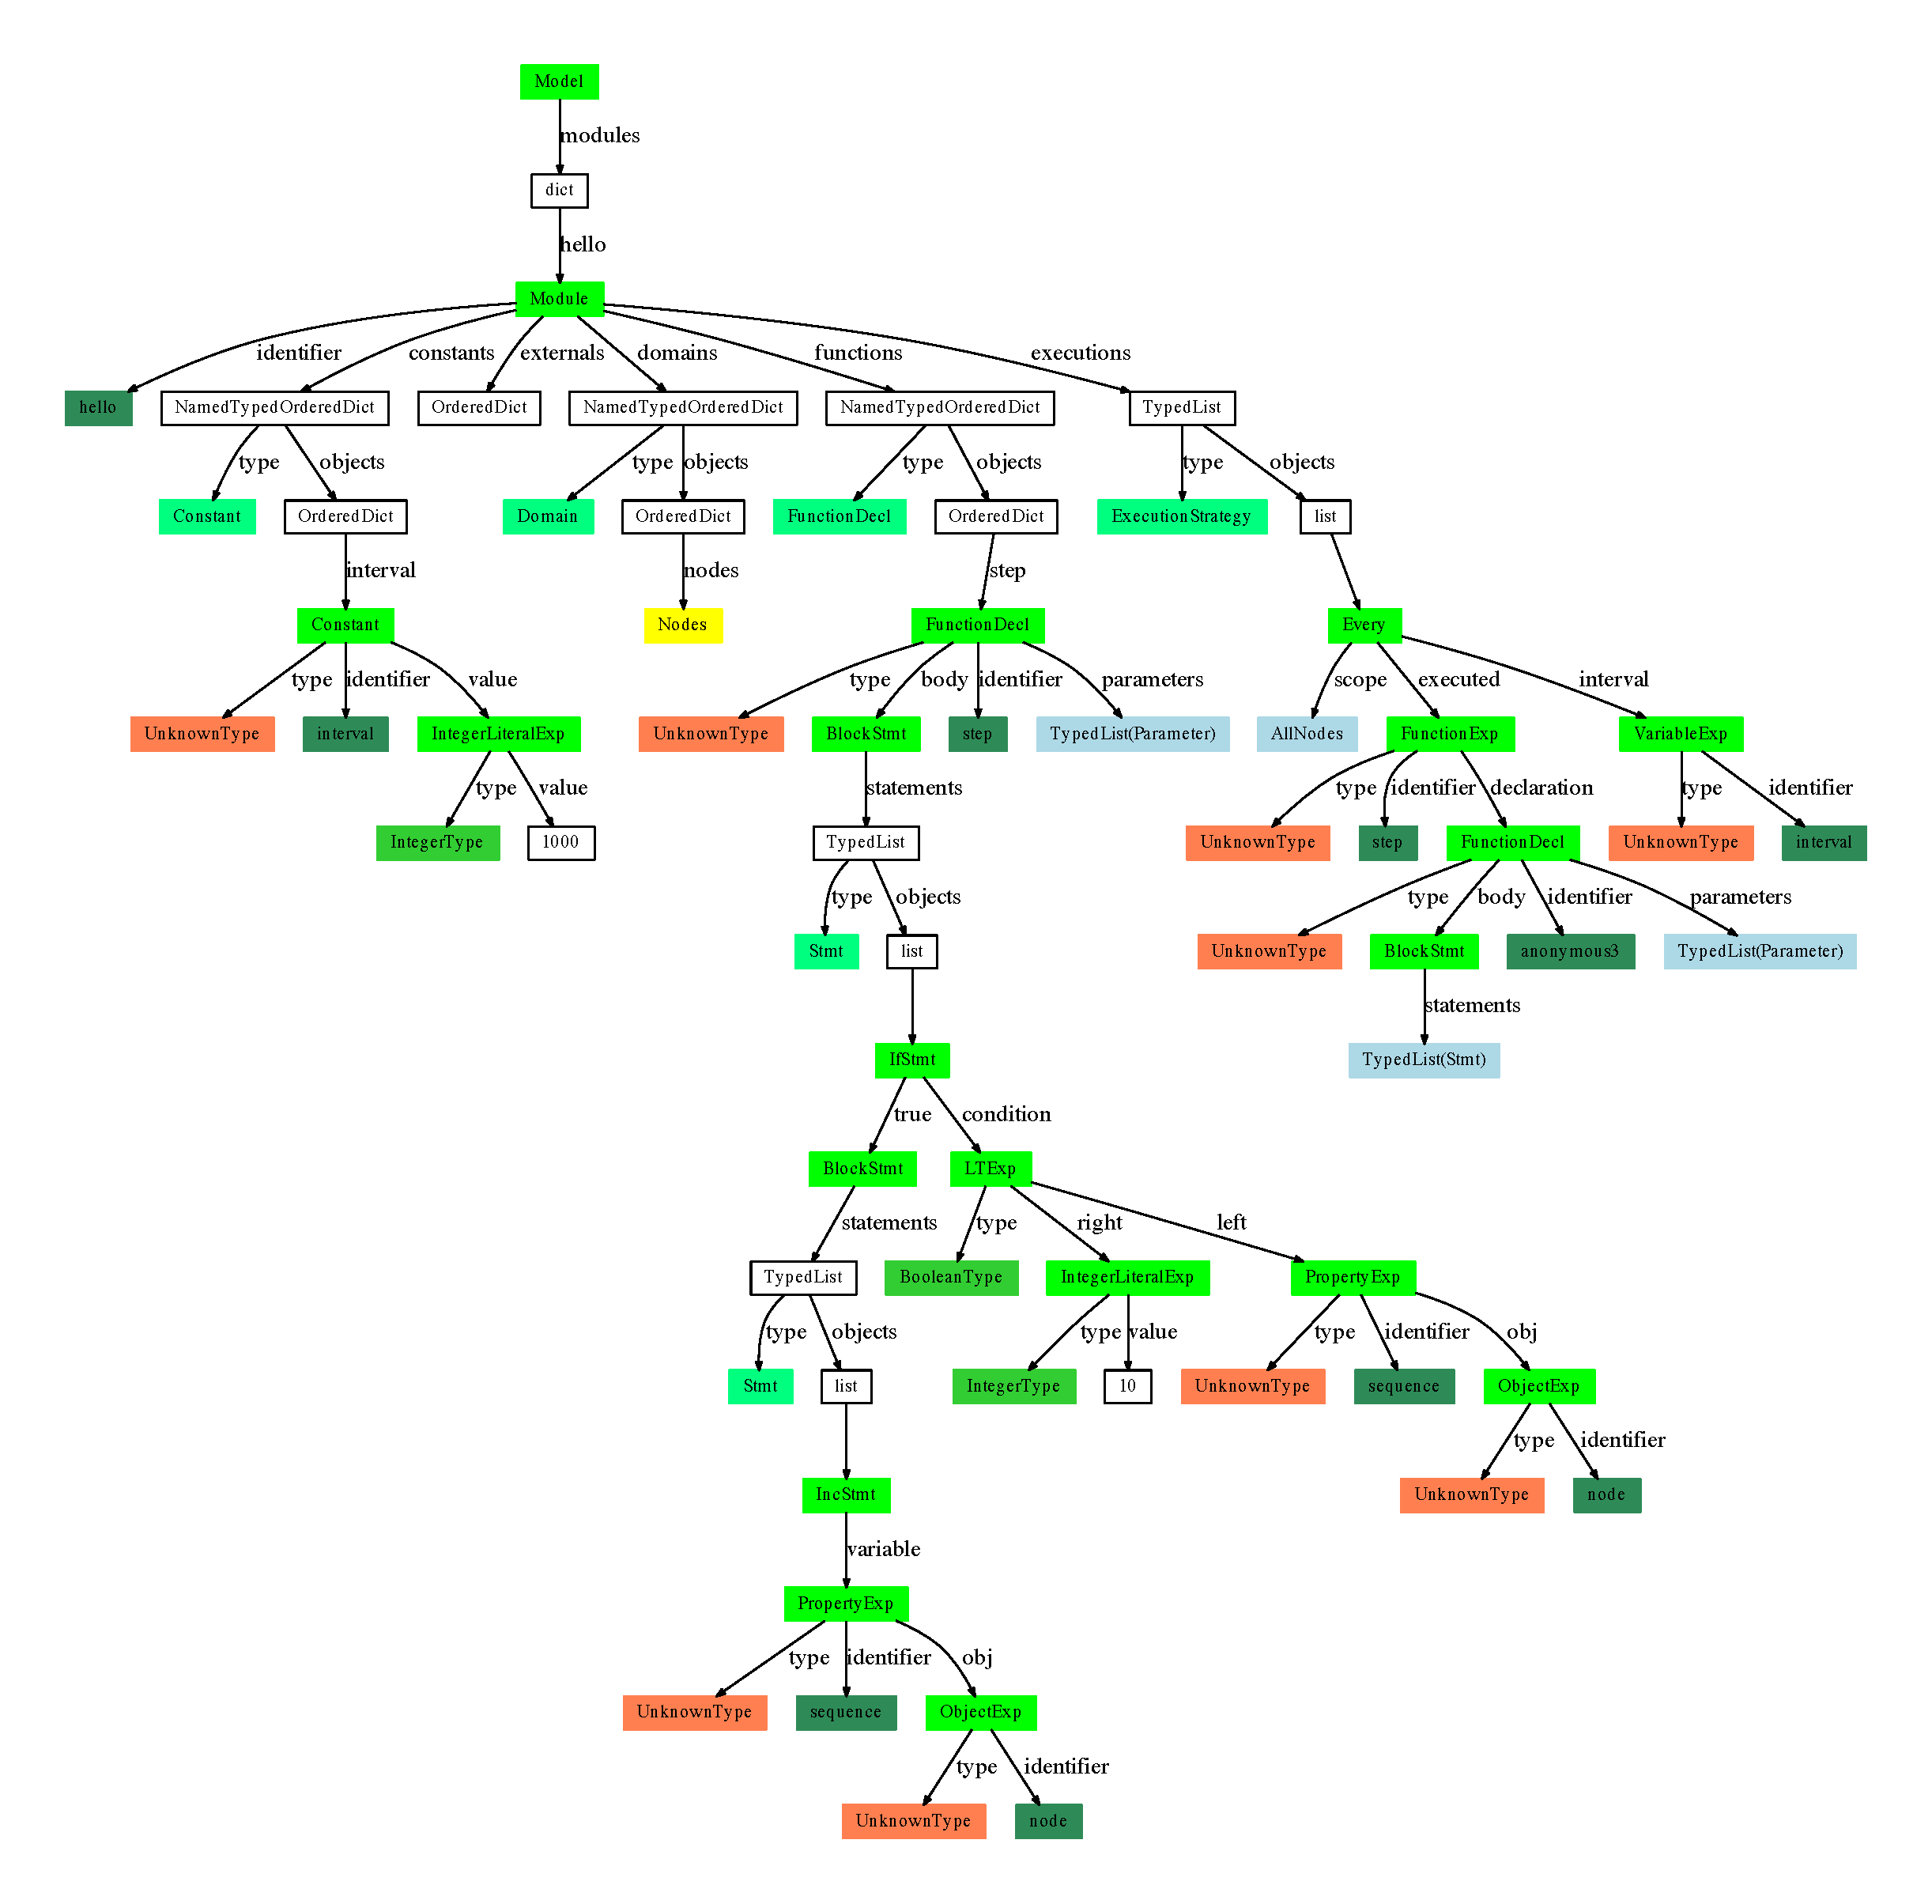
\includegraphics[width=\linewidth]{resources/hello_sm.pdf}
  \caption{Het SM van het elementaire voorbeeld, \ttt{hello.foo}}
  \label{fig:hello.sm}
\end{figure}

Het SM bevat meer informatie dan de AST, zoals bv. typering. Bij deze
visualisatie is gebruikgemaakt van een kleurencodering. Hierdoor wordt het
makkelijker om het diagram te interpreteren.

De belangrijkste kleur is rood en geeft problemen in het model aan, zoals
onbekende types. Dit is in deze fase van het generatieproces normaal, aangezien
typering in FOO-lang optioneel is. Deze eerste versie van het SM bevat daarom
nog niet alle types.

Een ander deel dat lijkt te ontbreken in dit diagram is de uitbreiding van het
domein. In het voorbeeld werd immers een eigenschap \ttt{sequence} toegevoegd.
Aangezien dit een uitbreiding is van het domein, zal deze eigenschap terug te
vinden zijn in de instantie van het domein voor deze module. In figuur
\ref{fig:hello.sm} is dit domein beperkt tot een referentie in een gele kleur.
De volledige inhoud van wat hierachter schuilgaat, is opgenomen in bijlage
\ref{section:nodes.sm} en vormt een groot stuk van het SM. Het behelst
verschillende types en functiedeclaraties die door het \ttt{nodes}-domein
ge\"introduceerd worden. Hier vinden we de uitbreiding met de extra
\ttt{sequence}-eigenschap.

\vspace{-3mm}

\subsubsection{Typedeductie}

De volgende stap in het generatieproces bestaat erin om de nog onbekende types
te deduceren op basis van andere informatie uit het SM. Dit gebeurt aan de hand
van de \ttt{inferrer}-module. Dit is een implementatie van de \emph{visitor}
voor het SM die nagaat of alle types gekend zijn. Voor onbekende types wordt,
afhankelijk van de plaats van het type, op verschillende manieren op zoek
gegaan naar een juiste typering.

De eenvoudigste manier bouwt, terwijl het model doorlopen wordt, een overzicht
op van gekende types die ontstaan door de declaratie van variabelen\dots Indien
een onbekend type wordt gevonden, consulteert de \ttt{inferrer}-module dit
overzicht. Indien een referentie naar een eerdere declaratie gevonden wordt,
kan het type eenvoudig gededuceerd worden.

In een aantal gevallen is de deductie niet rechtstreeks af te lezen uit
declaraties en moet er naar andere mogelijke combinaties gekeken worden.
Voorbeelden hiervan zijn bv. functiedeclaraties die gebruikt worden als reactie
op een gebeurtenis. De gebeurtenis specificeert hoe de reagerende functie
gedeclareerd is. Op basis van de omkaderende gebeurtenis moet vervolgens het
overeenkomstige prototype van de functie opgezocht en gekoppeld worden.

Na het succesvol uitvoeren van deze typedeductie zijn alle voorheen onbekende
types gekend en is het model volledig. Figuur \ref{fig:hello.sm-inferred} toont
hetzelfde SM als voordien, echter nu met volledig gekende typering.

\begin{figure}[ht]
  \centering
  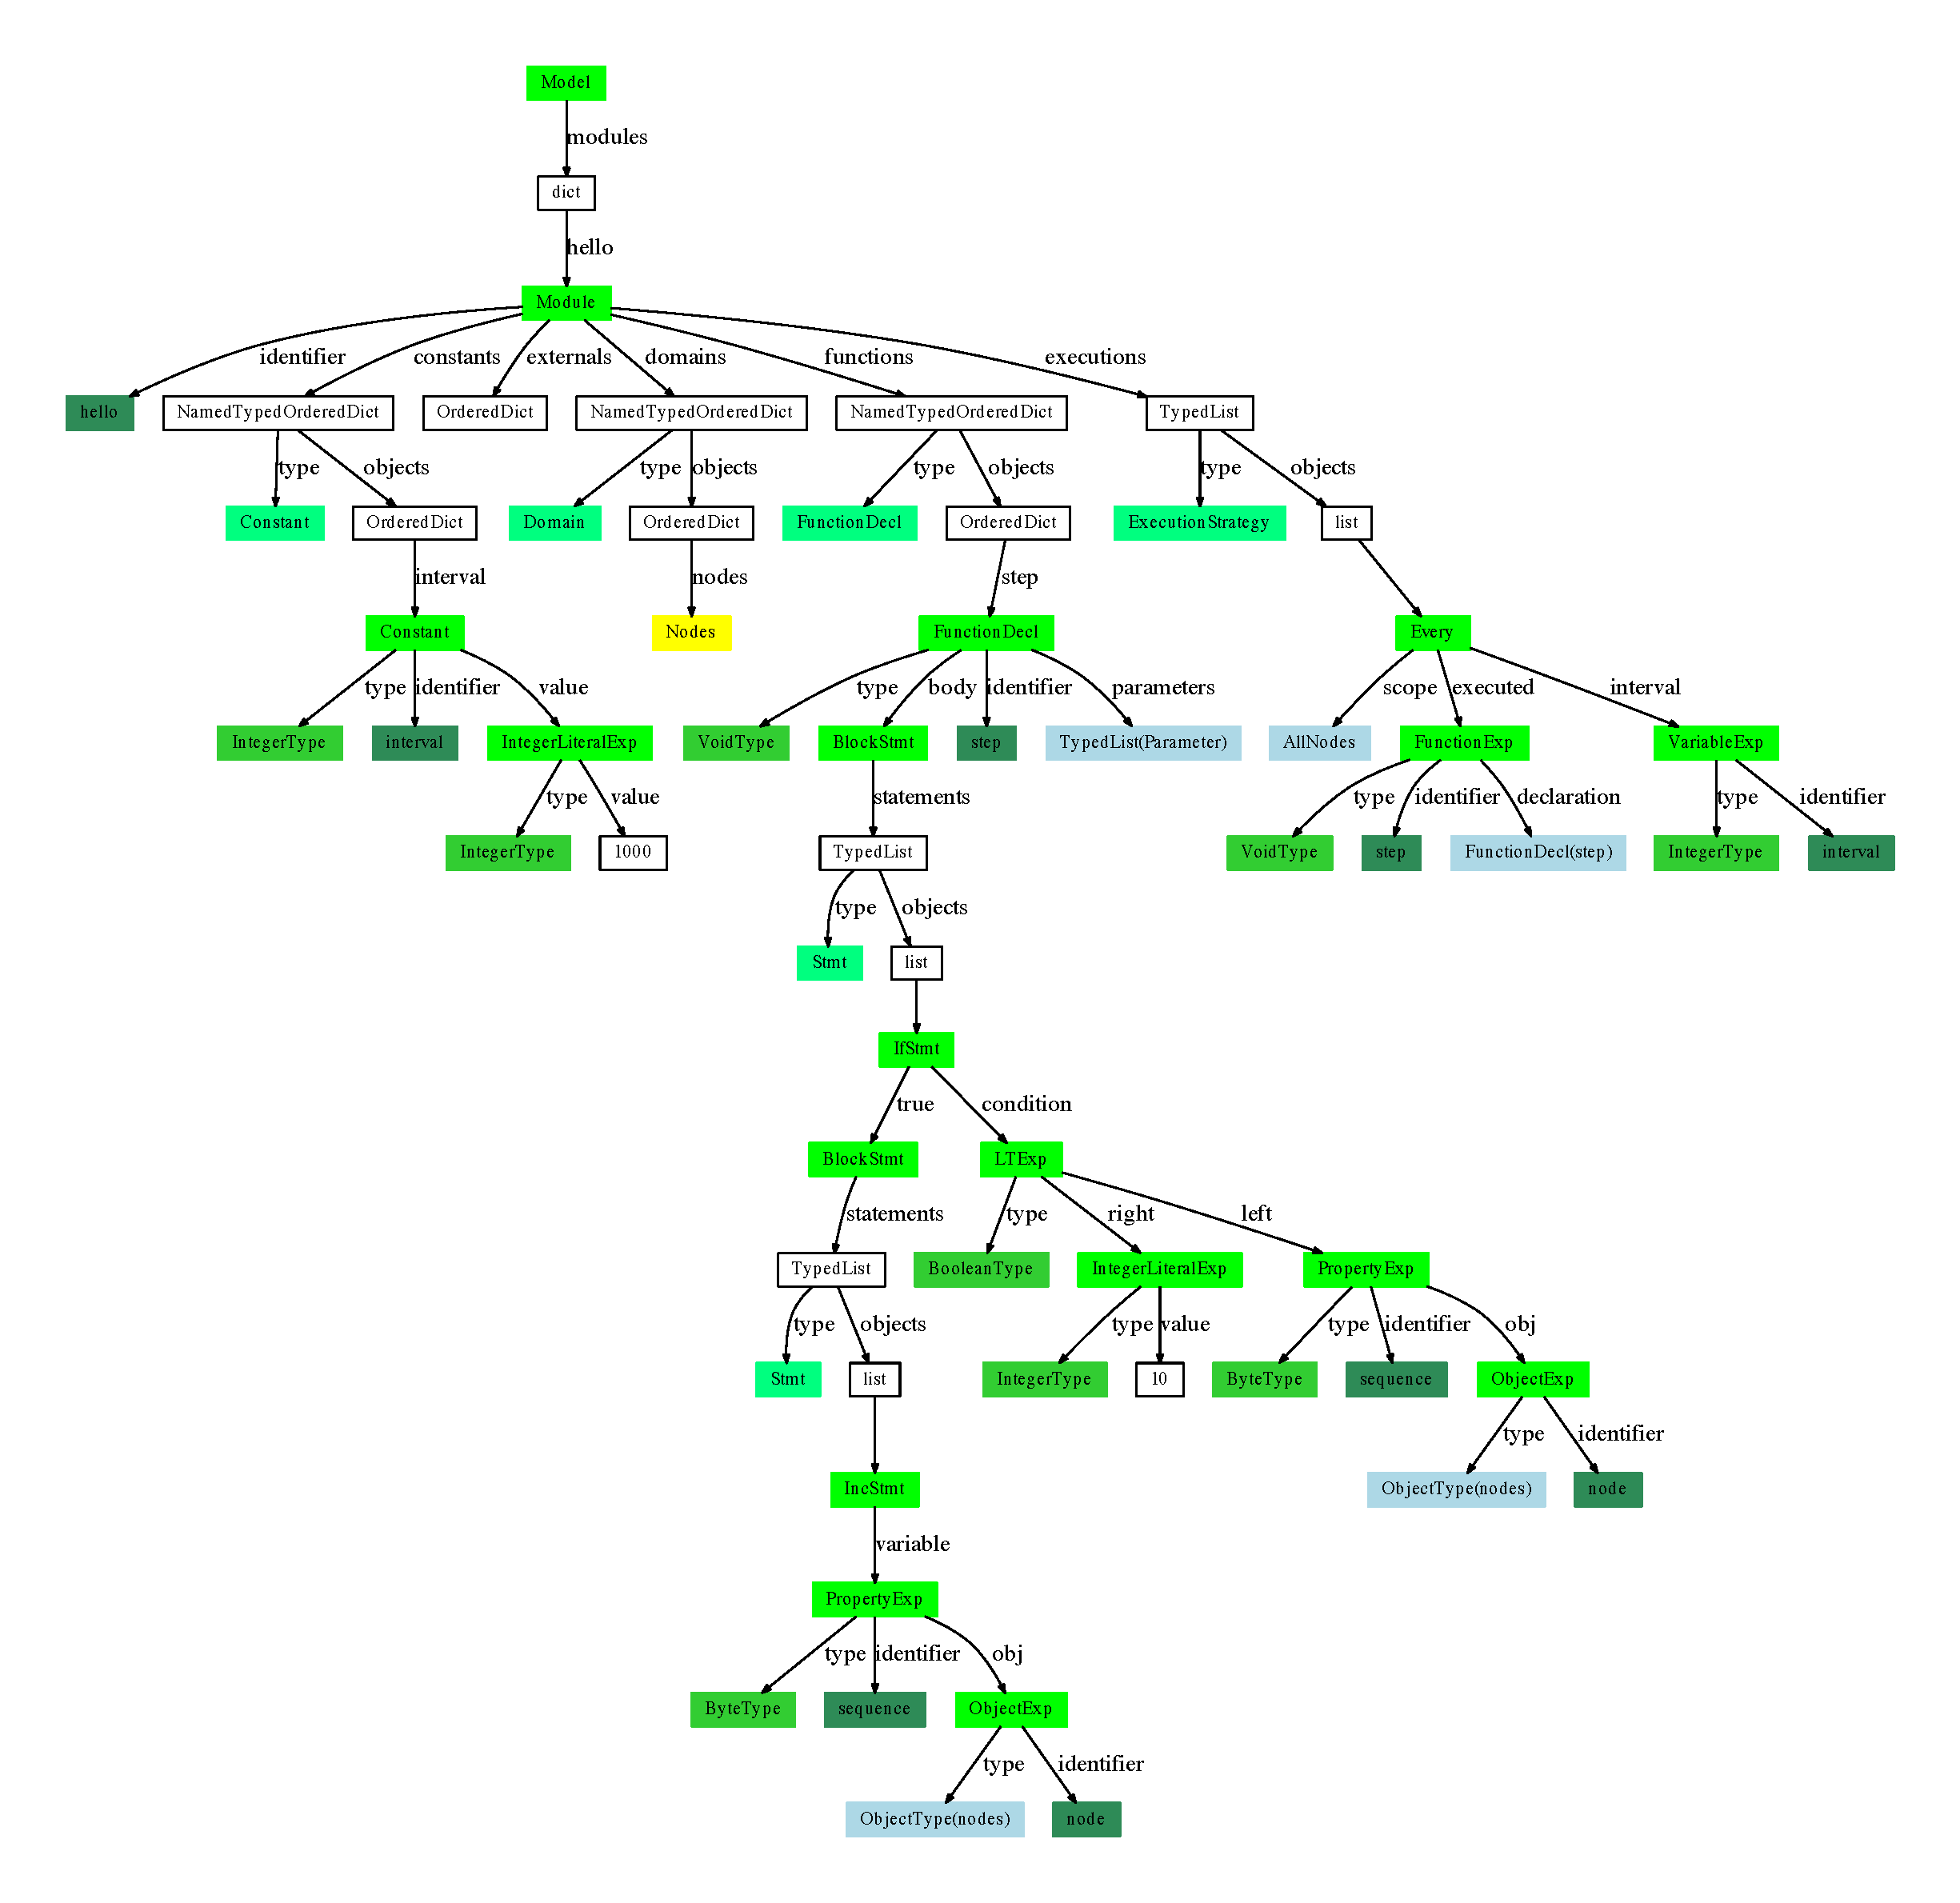
\includegraphics[width=\linewidth]{resources/hello_sm_inferred.pdf}
  \caption{Het SM van het elementaire voorbeeld, \ttt{hello.foo}, na type deductie}
  \label{fig:hello.sm-inferred}
\end{figure}

Ofschoon men verwacht dat deze fase geen structurele wijzigingen aanbrengt aan
het SM, zien we in dit geval toch dat er een vijftal elementen uit het model
verdwenen lijken te zijn. Dit is nochtans een gewoon voorbeeld van deductie. Na
het inladen van het initi\"ele model werd de (enige) uitvoeringsstrategie
gekoppeld aan een functie-expressie (\emph{FunctionExp}) genaamd \ttt{step}. Op
dat ogenblik was er over \ttt{step} niets geweten. De declaratie van \ttt{step}
was wel eerder gebeurd, maar het is pas in de deductiefase dat het onbekende
type van deze functie opgezocht werd. Deel van het type is tevens de declaratie
ervan. Tijdens de typedeductie wordt deze gekoppeld aan de declaratie, waardoor
in figuur \ref{fig:hello.sm-inferred} deze functiedeclaratie niet meer getoond
wordt, maar als een referentie naar de \ttt{step}-functie opgenomen is.

\vspace{-3mm}

\subsubsection{Modelcontrole}

De \ttt{inferrer}-module tracht alle onbekende types te deduceren. Een tweede
ondersteunende module is de \ttt{checker}-module of modelcontrole. Deze
overloopt aan de hand van een \emph{visitor} het hele model en controleert of
alles in orde is.

De \ttt{checker}-module is typisch nuttig bij het schrijven van FOO-lang code
en kan dienen als syntactische en semantische controle. Wanneer er bv. een
schrijffout gemaakt wordt in de naam van een variabele of functie, kan dit soms
niet direct opvallen. FOO-lang maakt bv. automatisch declaraties voor
variabelen aan wanneer zij voor het eerst gebruikt worden en nog niet eerder
gedeclareerd werden. De \ttt{checker}-module kan bv. voor deze situaties
waarschuwingen geven, die kunnen helpen bij het schrijven van de FOO-lang
broncode.
